
\documentclass[twoside]{protokoll}
\usepackage{graphicx}
\usepackage{tabularx} % for better table formatting
\usepackage{booktabs} % for better table formatting
\usepackage{float} % for preservint the order of figures and tables
\praktikum{I}
\usepackage{subfig}


\versuchsgebiet{(Akustik)}


\teilnehmer{Maximilian Carlos Menke, 434170}
\teilnehmer{Andrea Roth, 428396}
\gruppe{A3}

\begin{document}

\begin{versuchsziele}
Ziel des Versuches ist, das Elastizitätzsmodul verschiedener Metallstäbe zu bestimmen.
Eine statische Messung liefert nur für dünne Drähte Ergebnisse weswegen das Elastizitätsmodul in unserem Fall mit einer Dynamischen Messung bestimmt wird. Hierfür erzeugen wir stehende Wellen in den Metallstäben. So können wir mit der Frequenz und der Wellenlänge die Phasengeschwindigkeit und somit auch das Elastizitätsmodul bestimmen. 
\end{versuchsziele}

 
\section{1A3 Bestimmung des E-Moduls von Metallen}

\begin{aufgabe}{Grundlagen}
  % Knappe Beschreibung der theoretischen Grundlagen, Angabe der
  % Fbenötigten Formel(n), ohne Herleitung. Definition der verwendeten
  % Formelzeichen.
    Da wir keine Statische Messung des E-Moduls durchführen können, verwenden wir hier eine dynamische Messung.
    Für diese brauchen wir Grundlagen aus der Akustik über stehende Wellen, als auch von Festkoerpern.


    Das E-Modul ist ein Maß für die Dehnbarkeit eines Materials. Es ist Definiert als: 
    \begin{equation}
        E = \frac{\frac{F}{A}}{\frac{\Delta L}{L}}
    \end{equation}
    Es beschreibt wie sehr sich ein Material aus dehnt / komprimiert wenn ein Druck auf ihn ausgeübt wird.
    Es gilt allerdings nur im elastischen Bereich des Materials.\\
    
    Wenn wir mit dem Hammer auf das Ende des Stabes schlagen, so ensteht eine Druckwelle in ihm.
    Diese durchläuft den Stab. Am andren Ende des wird dieser ein kleines Stück ausgedehnt.
    Dieses sorgt dafür, das die Druckänderungen an die Luft übertragen wird.
    Da der Stab aber ein Elastizitätsmodul besitzt, gibt es eine Rückstellkraft die die Ausdehnung des Stabes wieder zurückführt.
    Diese Druckschwankung durchläuft den Stab periodisch.
    Dadurch entsteht eine Stehende Welle in dem Stab, welche über die Enden des Stabes Schallwellen an die Umgebung abgibt.

    Wenn der Stab in Schwingung versetzt wird, bliden sich stehende Wellen in ihm aus.
    Wir wollen hierbei die Frequenz der Grundschwingung bestimmen.
    Da der Stab an beiden Enden ein festes Ende für die Wellen hat, muss für Resonanz der Grundschwingung die Wellenlaenge: $\lambda = 2 L$. 
     
    Daraus ergibt sich:
    \begin{equation}
        v = f \lambda = f 2 L
    \end{equation}

    In Luft breitet sich Schall immer als Longitudinale Welle aus.
    In Festkörpern muss die Rückstellkraft des Materials nicht zwangsweise entgegen der Ausbreitungsrichtung zeigen, weshabl hier allgemein auch eine Transversalve Komponenten vorliegen kann.
    Die Metallstäbe können aber als homogen genung angenommen werden, weshalb wir hier von einer longitudinal Welle ausgehen können.
    Aus der Wellengleichung ergibt sich:
    \begin{equation}
         v = \sqrt{\frac{E}{\rho}}
    \end{equation}
    \begin{equation}
         E = v ^2 \rho
    \end{equation}
    \begin{equation}
        E = (f \lambda)^2 \rho = 4 f_0 L ^2 \rho
    \end{equation}
    \begin{equation}
        E = f \lambda = \frac{ 4 f_0^2 L ^2 M}{\pi (\frac{d}{2}) ^2}
    \end{equation}
    \begin{equation}
        E = f \lambda = \frac{ 16 f_0^2 L ^2 M}{\pi d ^2}
    \end{equation}

     
\end{aufgabe}

\begin{aufgabe}{Versuchsaufbau und Versuchsdurchführung}
\subsection{Versuchsaufbau}
  Für die Bestimmung des E-Moduls messen wir die Schallwellen die mithilfe eines Gummihammers in dem Stab erzeugt wurden.
    Diese werden in ein Digitales Signal umgewandelt das wir mithilfe des Sensor CASSY darstellen können und analysieren.
    Hierzu benötigen wirfolgende Geräte.\\

    Für die Bestimmung des E-Moduls messen wir die Schallwellen die mithilfe eines Gummihammers in dem Stab erzeugt wurden.
    Diese werden in ein Digitales Signal umgewandelt das wir mithilfe des Sensor CASSY darstellen und analysieren können.
    Hierzu benötigen wir folgende Geräte.\\

\textbf{Benötigte Geräte:}
\begin{itemize}
\item Semsor CASSY
\item Universalmikrofon mit Stativstange
\item Sockel
\item Tischklemme
\item Metallstange (Länge: 20cm) (Stativstange für Kreuzmuffe)
\item Kreuzmuffe
\item Metallstift (Qürschnitt: 4mm, Länge: 30mm)
\item Gummi-Hammer
\item Mikrometerschraube (Messbereich: 0-25mm, Genauigkeit: $\pm$ 0.01mm)
\item Stahl-Bandmaß (Länge: 2m, Tolleranz: $\pm$ 0.7mm)
\item verschiedene Metallstangen (Kupfer, Messing, Stahl, Aluminium)
\item Analysewaage Sartorius BL 1500 (Genauigkeit: $\pm$ 0,2g)
\end{itemize}


\begin{figure}[H]
  \centering
  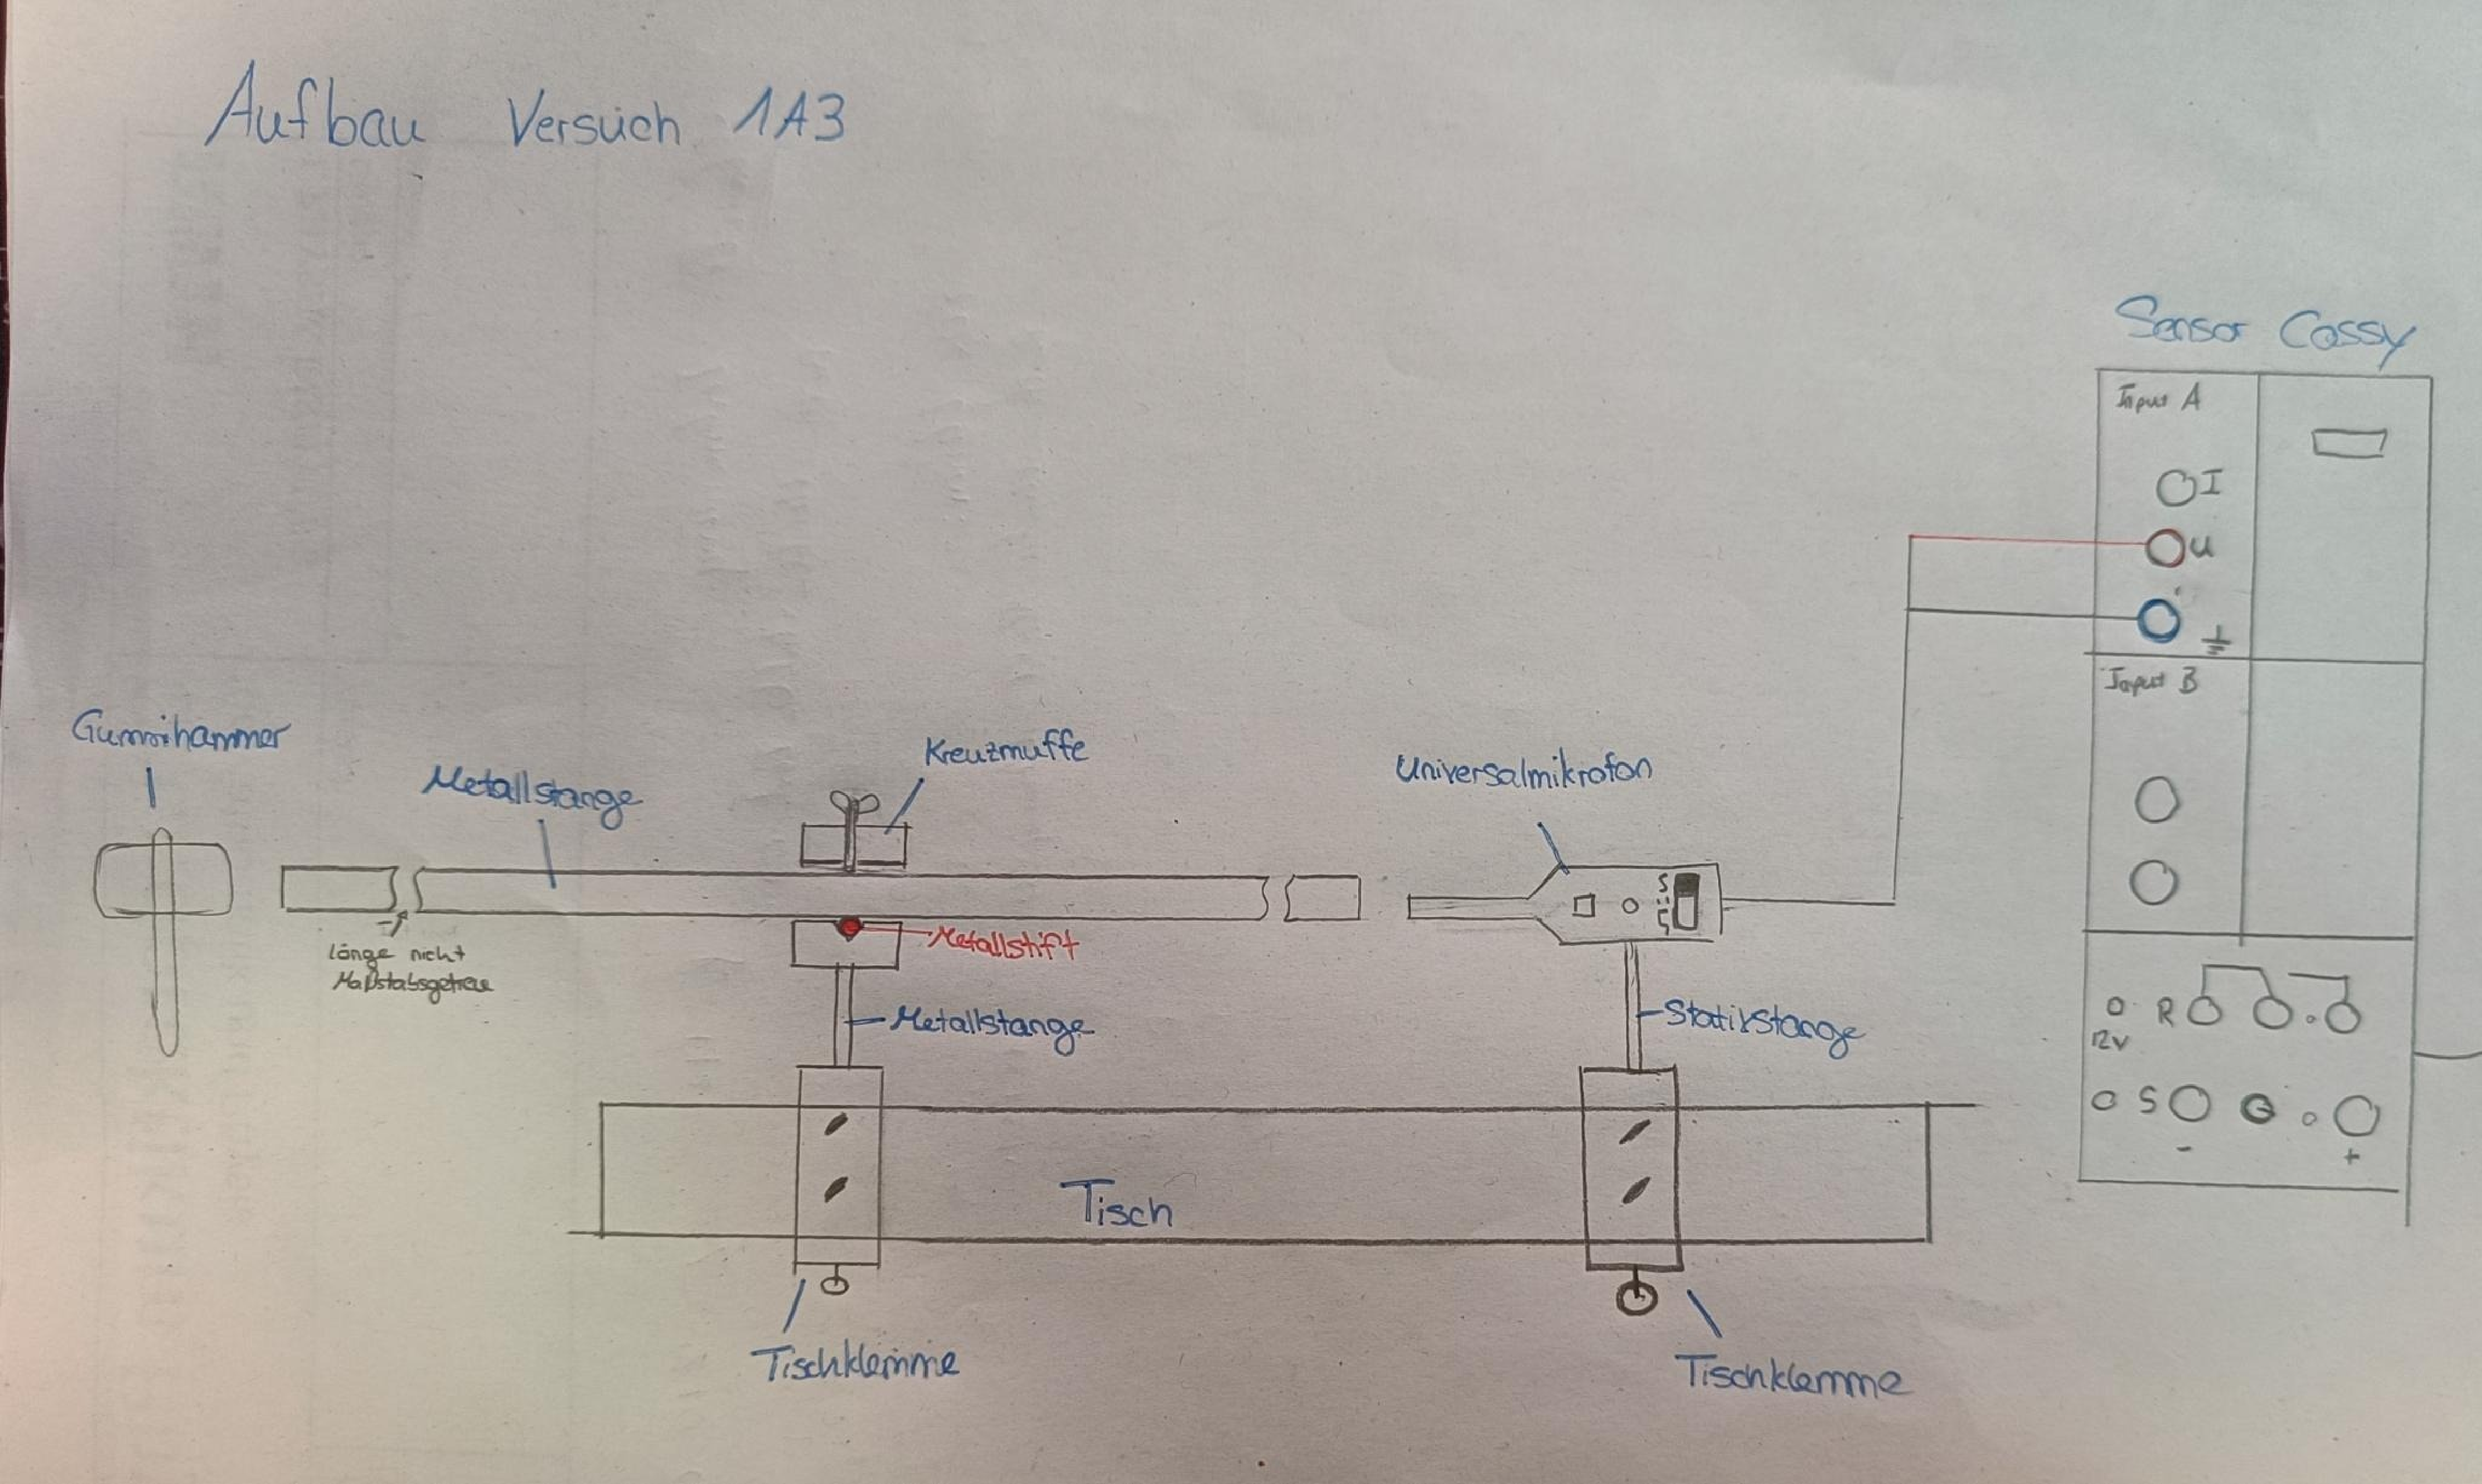
\includegraphics[width=0.8\textwidth]{Bilder/434170_428396_1A3_SkizzeAufbau.pdf}
  \caption{Skizze des Versuchsaufbaus}
  \centering
\end{figure}
 
Der Aufbau des Experiments kann der oben stehenden Skizze entnommen werden. 

Zunächst werden mit zwei Tischklemmen Mikrofon und Metallstange an dem Tisch befestigt. Wobei die Stange mithilfe der Kreuzmuffe befestigt wird. In die Kreuzmuffe wird der Metallstift ortogonal zu der Stange hineingelegt, sodass diese beim mittigen einspannen nur an einem Punkt unterstütz wird. Die Stange also frei schwingen kann. 

Das Universalmikrofon und die Metallstange werden auf eine Linie gebracht, mit 5mm Abstand. Sodass Das Mikrofon die Schallwellen gut aufzeichnen kann, aber nicht beschädigt wird, falls die Stange zu stark angeschlagen wird. Wärend der gesamten durchführung muss darauf geachtet werden, dass die Position der beiden sich nicht gegeneinander verschieben. 


Das Universalmikrofon wird in den Sensor CASSY eingesteckt, wobei das Gelbe Kabel(in der Skizze rot) in die Buxe für die Spannung, und das schwarze in die für die Erdung gesteckt wird. Das Mikrofon wird auf den Amplitudenmodus $\sim$ gestellt. Der Gummihammer wird verwendet um auf das, dem Mikrofon abgewandte, Ende der Metallstange zu schlagen. Damit werden die Metallstangen zum schwingen angeregt.

\subsection{Durchführung}

Zunächst haben wir die Metallstangen kathegorisiert nach dem Material aus welchem sie gemacht sind.

\begin{itemize}
\item Aluminium:		 matt silberne stange 
\item Messing:		 goldene Stange
\item Kuper:			 kupferfarbene Stange
\item Stahl 15:		 silber glänzende Stange
\end{itemize}

Von diesen haben wir dann jewails, Länge, Masse und Durchmesser bestimmt. 
Die Länge haben wir mit dem Bandmaß gemessen, wobei hier darauf geachtet wurde, dass das Bandmaß straff ist. Die Masse haben wir mit der Analysewage bestimmt, indem wir die Stange mittig auf der Wage plaziert haben. 


Da wir bei der Stange annehmen, dass diese einen kreisförmigen querschnitt hat, was nicht perfekt zutreffen wird, führen wir die Messung des Durchmessers mehrfach durch. Hierfür verwenden wir die Mikrometerschraube. Wir messen an verschiedenen Stellen, dabei rotieren wir die Stange beliebig bei jeder Messung um die längsachse. Dies wiederholen wir zehn mal. Sodass wir für jede Stange 10 Messwerte für den Durchmesser haben.\\ 

\begin{figure}[H]
  \centering
  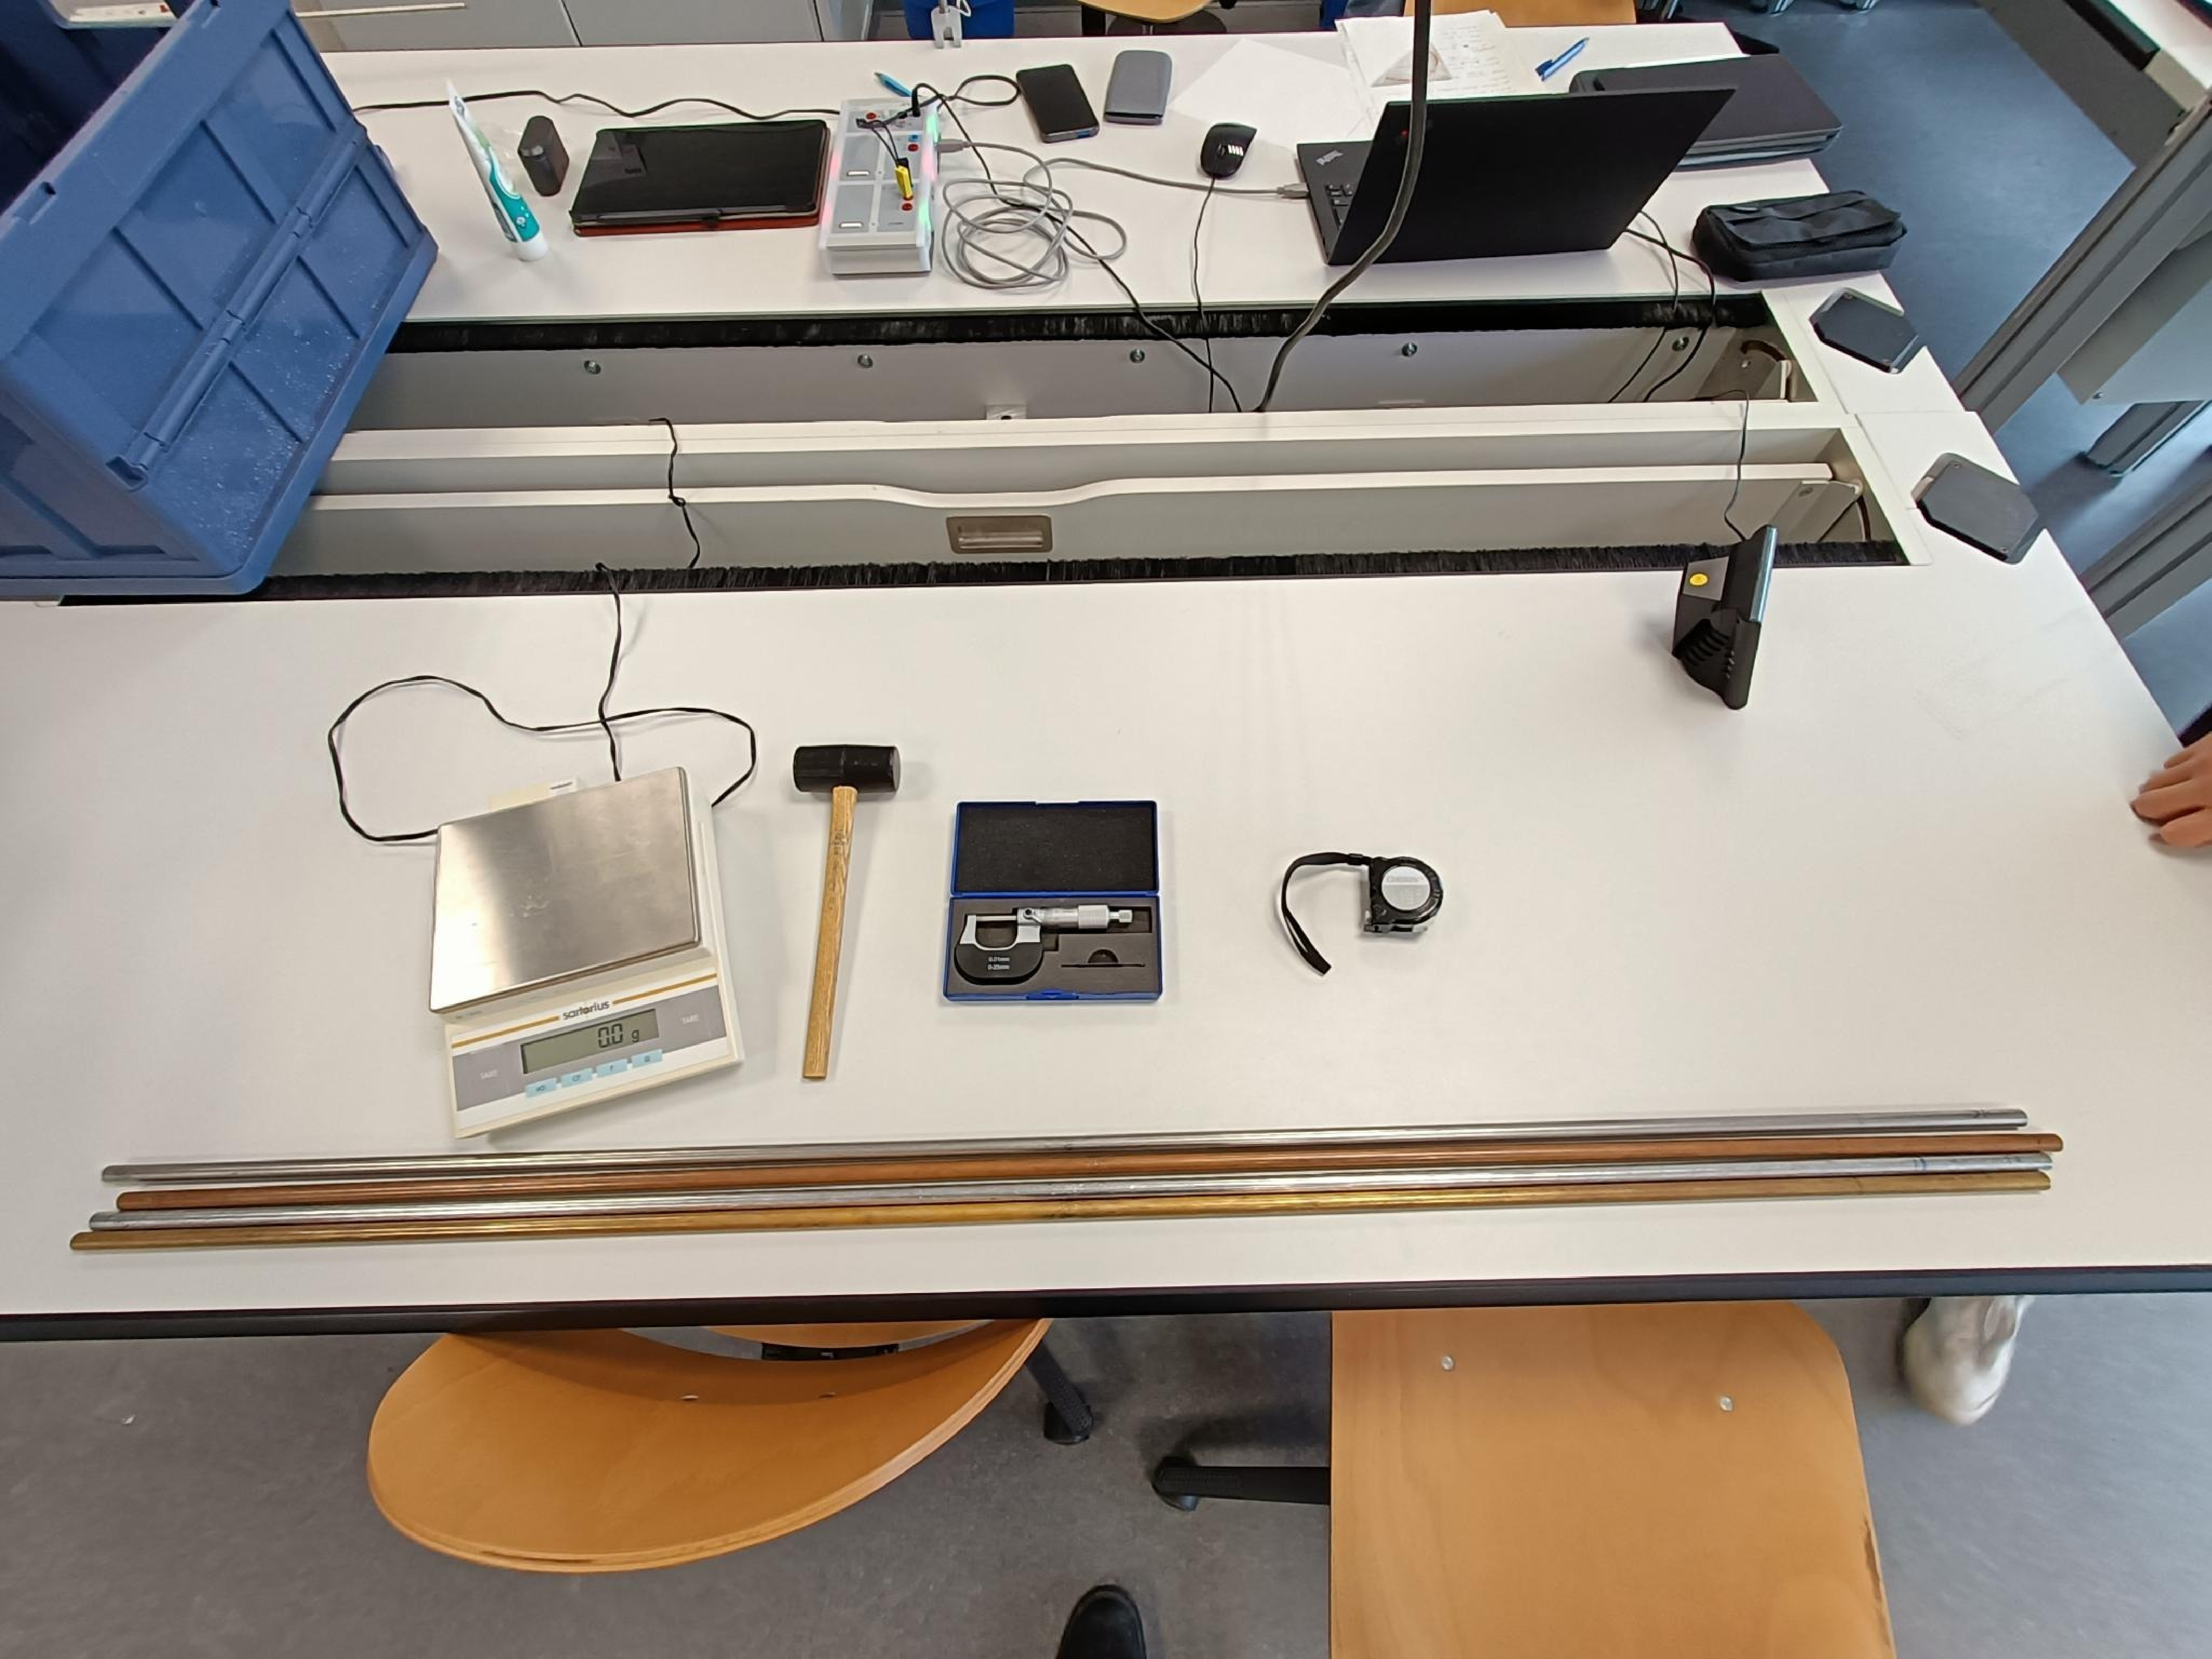
\includegraphics[width=0.8\textwidth]{Bilder/434170_428396_1A3_Materialien.pdf}
  \caption{Bild der Messgeräte und Metallstangen}
  \centering
\end{figure}

Als nächstes bauen wir den Versuch auf. Hier gehen wir genau so vor wie in der vorherigen beschreibung des Versuchsaufbaus. Als erstes haben wir die Kupferstange verwendet.
Wobei wir zunächst die Tischklemme plaziert haben und die Stange mittig eingespannt. Hierfür haben wir von einem Ende der Stange auß, mit dem Maßband die Mitte bestimmt. Dann haben wir das Mikrofon passend zu der Stange positioniert, und an den Tisch montiert. Hierbei haben wir noch beachtet, dass die Stange nicht zu fest eingespannt werden sollte, da dies auswirkung auf die Frequenz hat. Außerdem haben wir überprüft, dass sie nur an einem Punkt aufliegt, sodass sie frei schwingen kann. Die Spitze des Mikrofons haben wir ungefähr 5mm entfernt vom Ende der Stange positioniert. Dies haben wir nach Augenmaß getan. 

\begin{figure}[H]
  \centering
  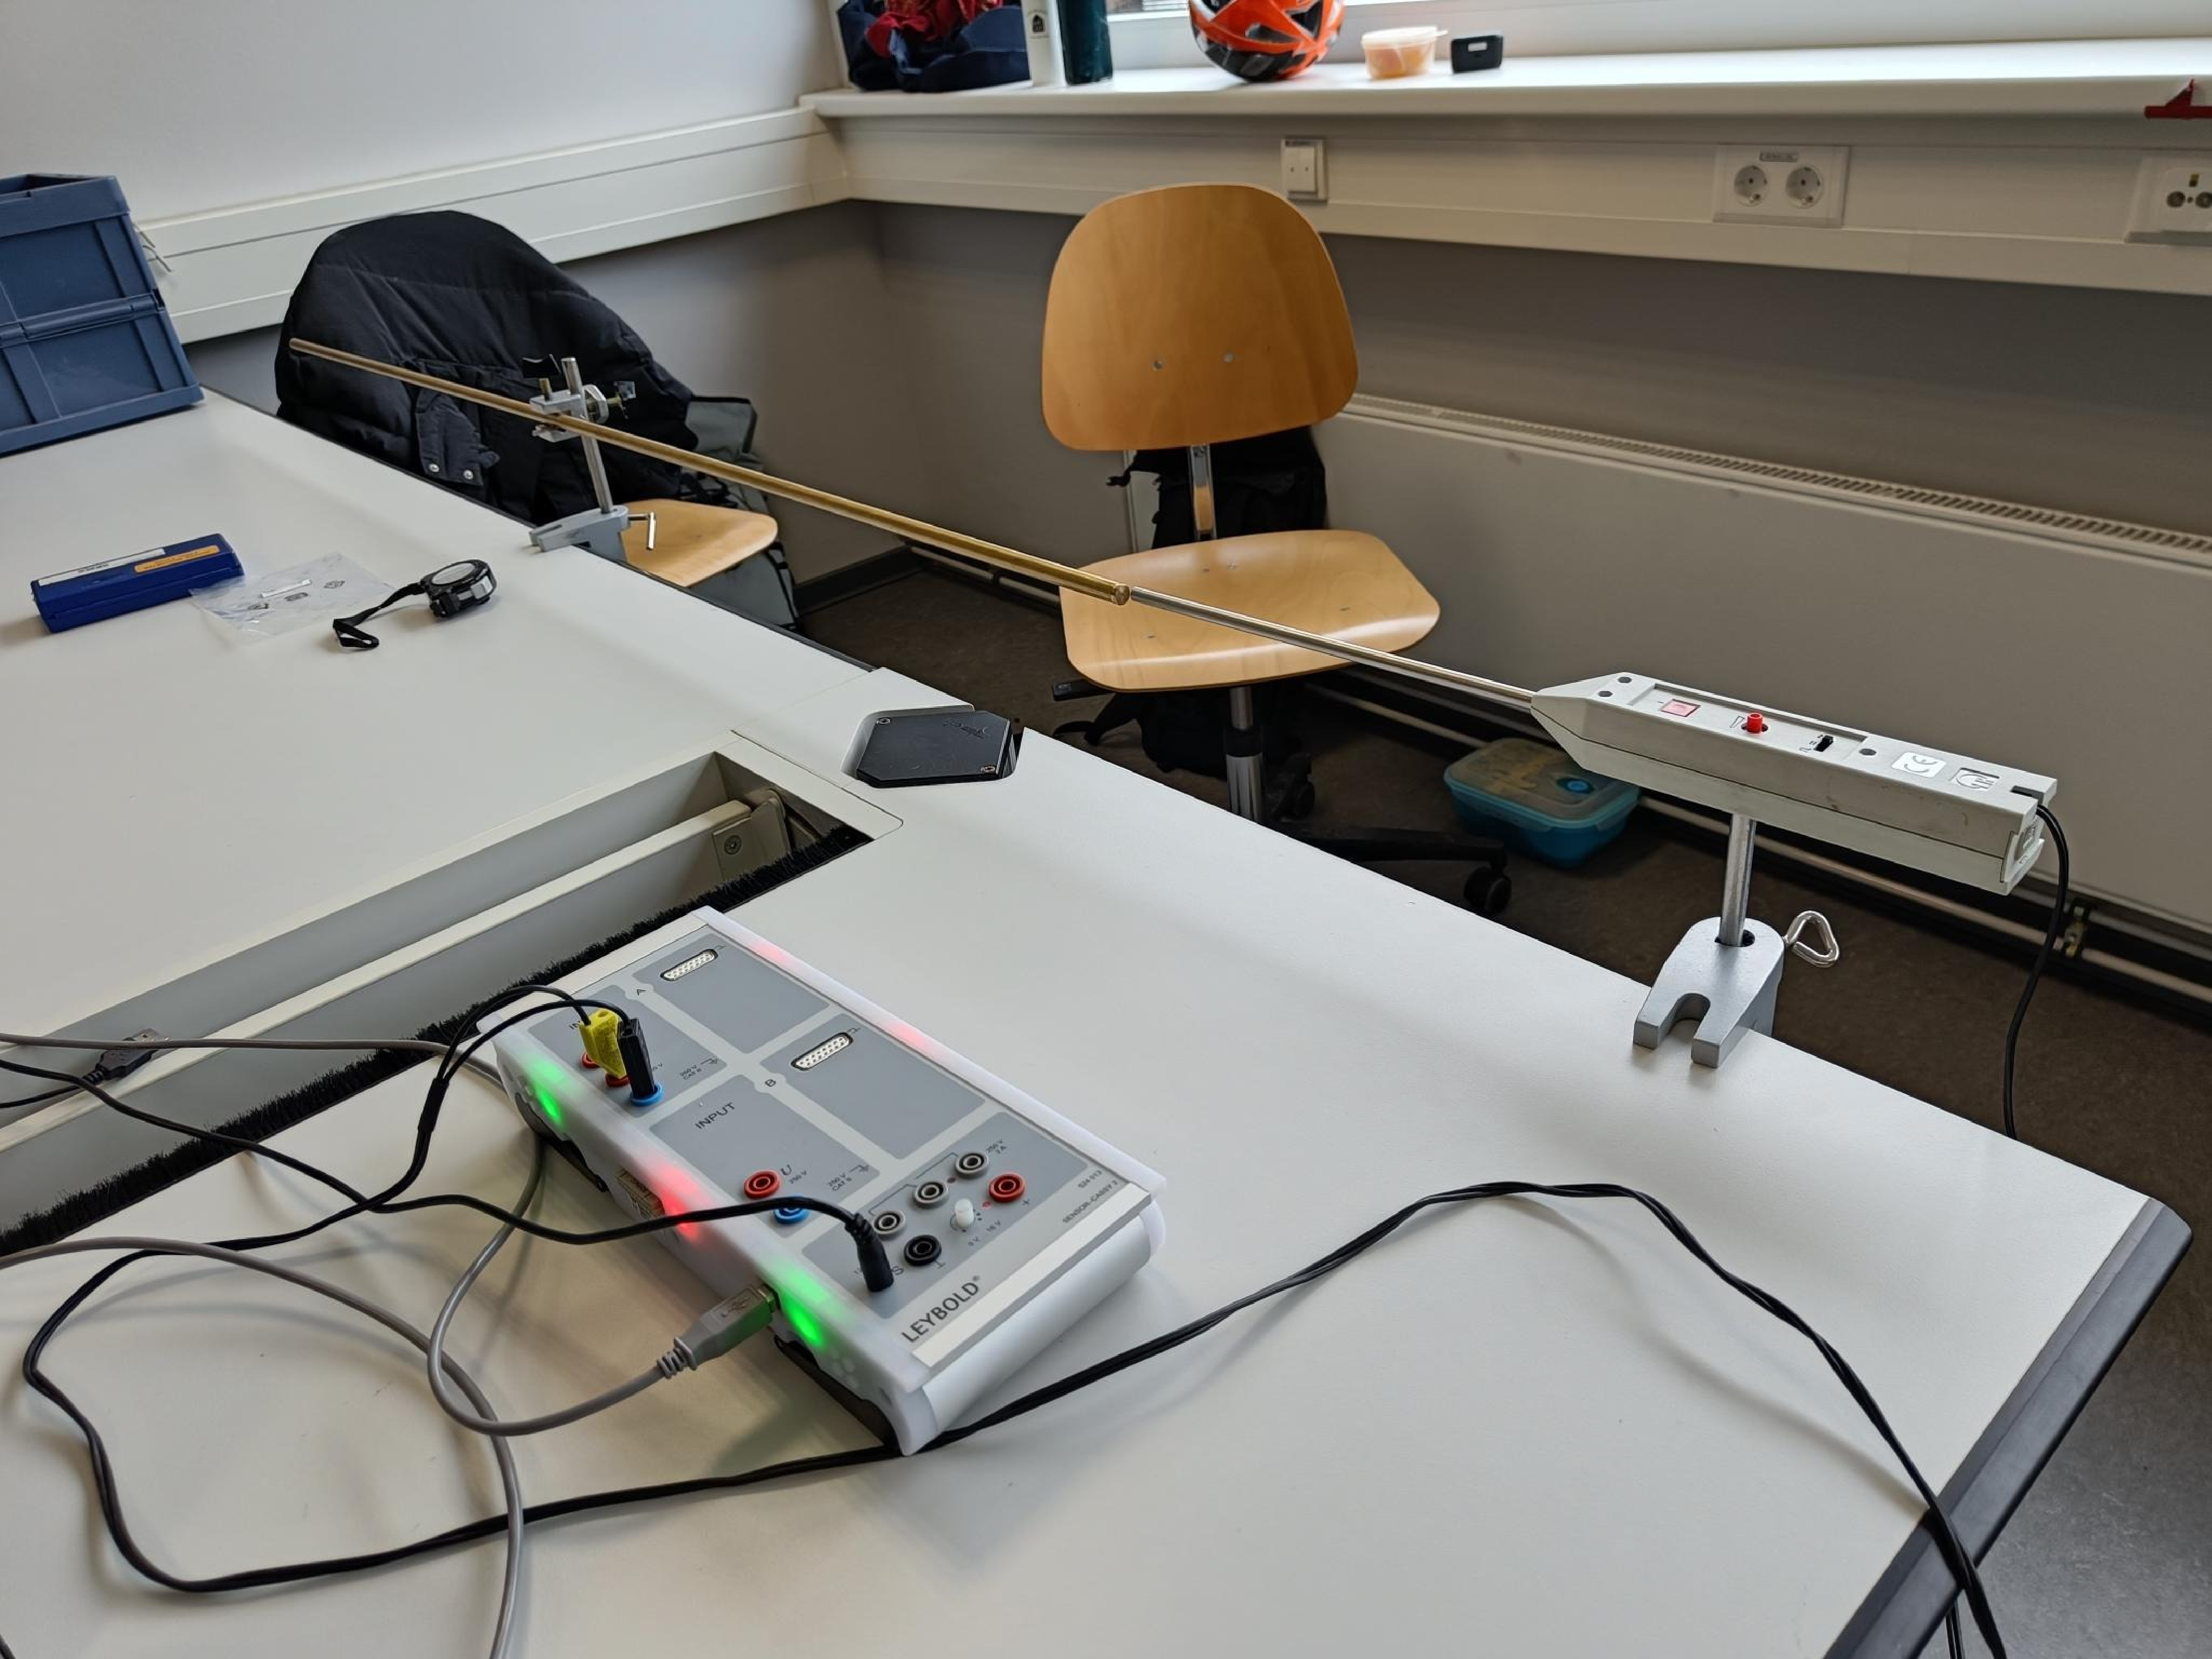
\includegraphics[width=0.8\textwidth]{Bilder/434170_428396_1A3_Gesamtaufbau.pdf}
  \caption{Bild der fertig aufgebauten Versuchsanordnung}
  \centering
\end{figure}

Dann haben wir das Mikrofon wie im Aufbau beschrieben an das Sensor Cassy angeschlossen und in betrieb genommen. Zunächst haben wir uns überlegt, was sinnvolle Messparameter sind. Da die Schallgeschwindigkeit in Metallen im bereich von mehrere 1000m/s liegt, muss das Messintervall im bereich von 10-100$\mu$s sein. Somit haben wir erste Testmessungen durchgeführt. Wobei wier diese mehrfach wiederholt haben, bis wir die Empfindlichkeit des Mikrofons so eingestellt hatten, dass wir den gesamten dynamischen bereich des Mikrofons ausnutzen, und nicht in die Sättigung kommen. Dann konnten wir eine erste FFT mit CASSY durchführen, und mit peakfinder die Frequenz des schwingenden Kupferstabs ungefähr bestimmen. Mit diesen Informationen haben wir dann unsere Messparameter eingestellt.\\

\textbf{Messparameter:}
\begin{itemize}
\item Messzeit: 3s
\item Intervall: 100$\mu$s
\item Anzahl Messungen: 30001
\item Spannungsbereich: -3V bis 3V (Da der dynamisch Bereich des Mikrofons 2.5V ist)
\end{itemize}

Wir haben für die Messung keinen Trigger verwendet, sondern die Messung manuell gestartet. 


Bei einer Messung hat einer aus unserer Gruppe mit dem Gummihammer den Kupferstab angeschlagen, wärend die andere Person kurz nach Anschlag die Messung gestartet hat, so dass, der Einschwingvorgang möglichst nicht mit aufgezeichnet wurde. Wir haben versucht den stab immer möglichst gleich an zu schlagen, also gleiche position und Kraft, damit die Messungen möglichst vergleichbar sind. Außerdem haben wir darauf geachtet, dass wir die Stange nur dann anschlagen, wenn niemand anders eine Stange des gleichen Materials anschlug.

\begin{figure}[!tbp]
  \centering
  \subfloat[Flower one.]{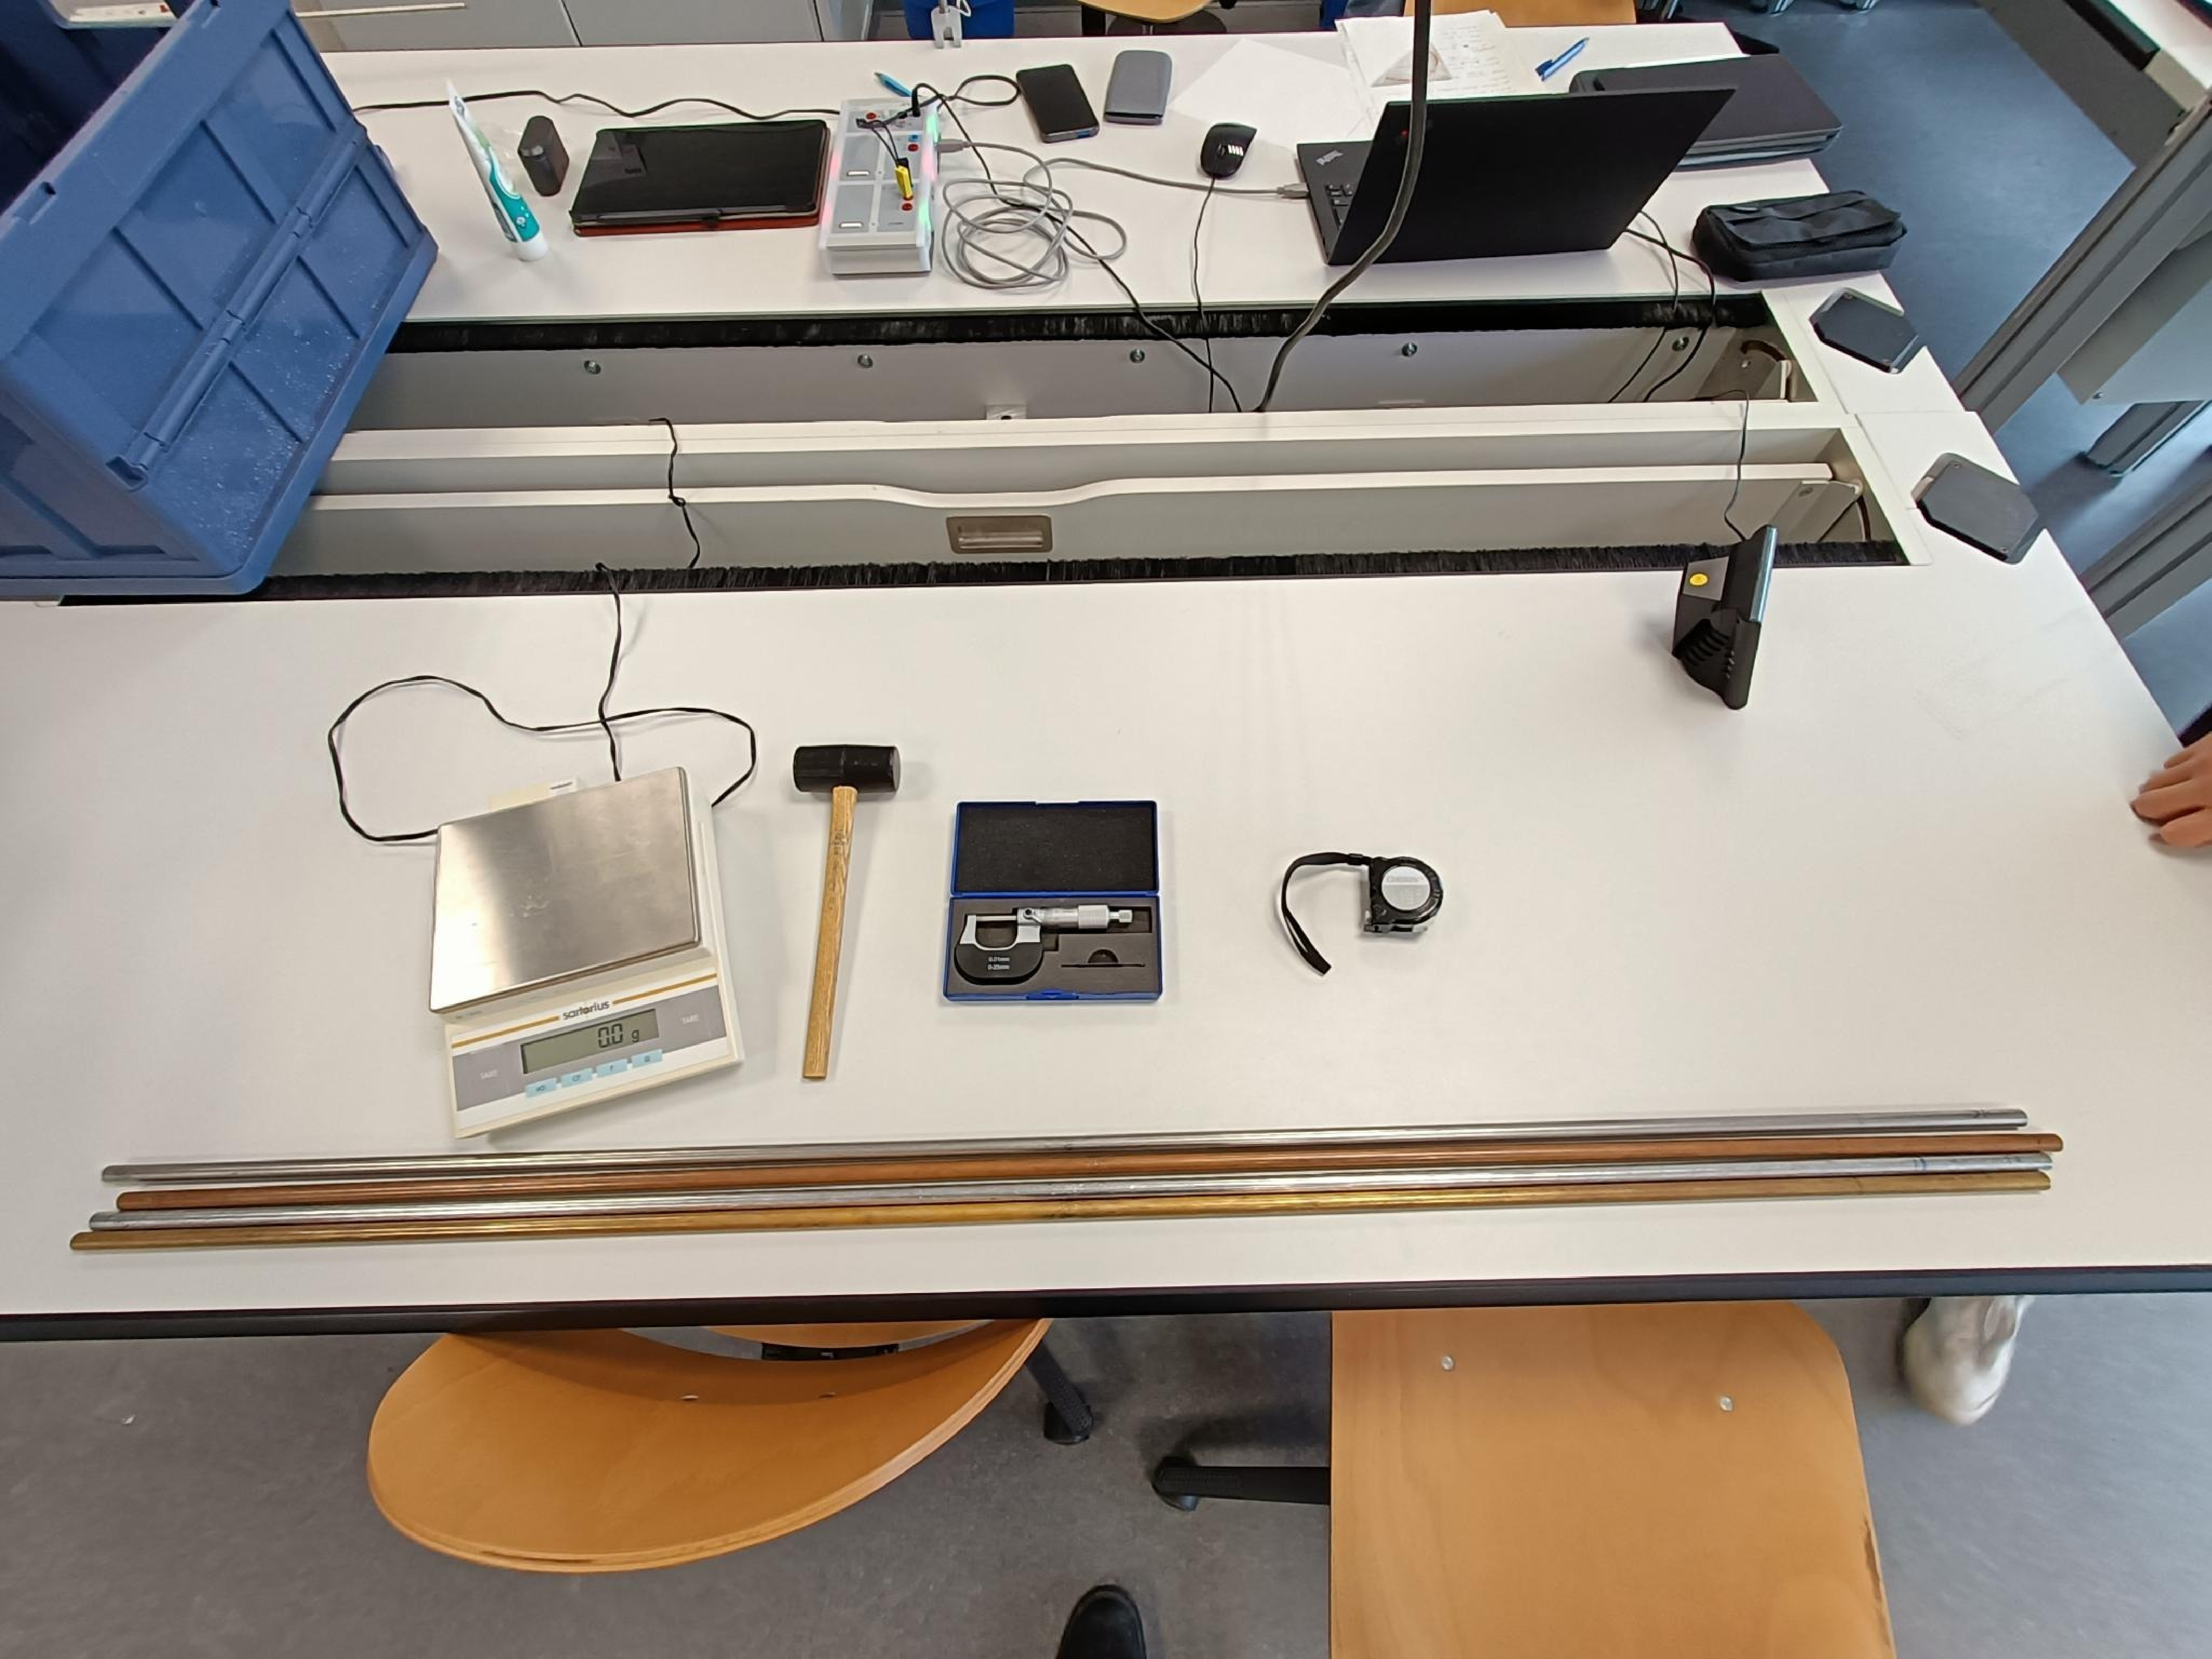
\includegraphics[width=0.3\textwidth]{Bilder/434170_428396_1A3_Materialien.pdf}\label{fig:f1}}
  \hfill
  \subfloat[Flower two.]{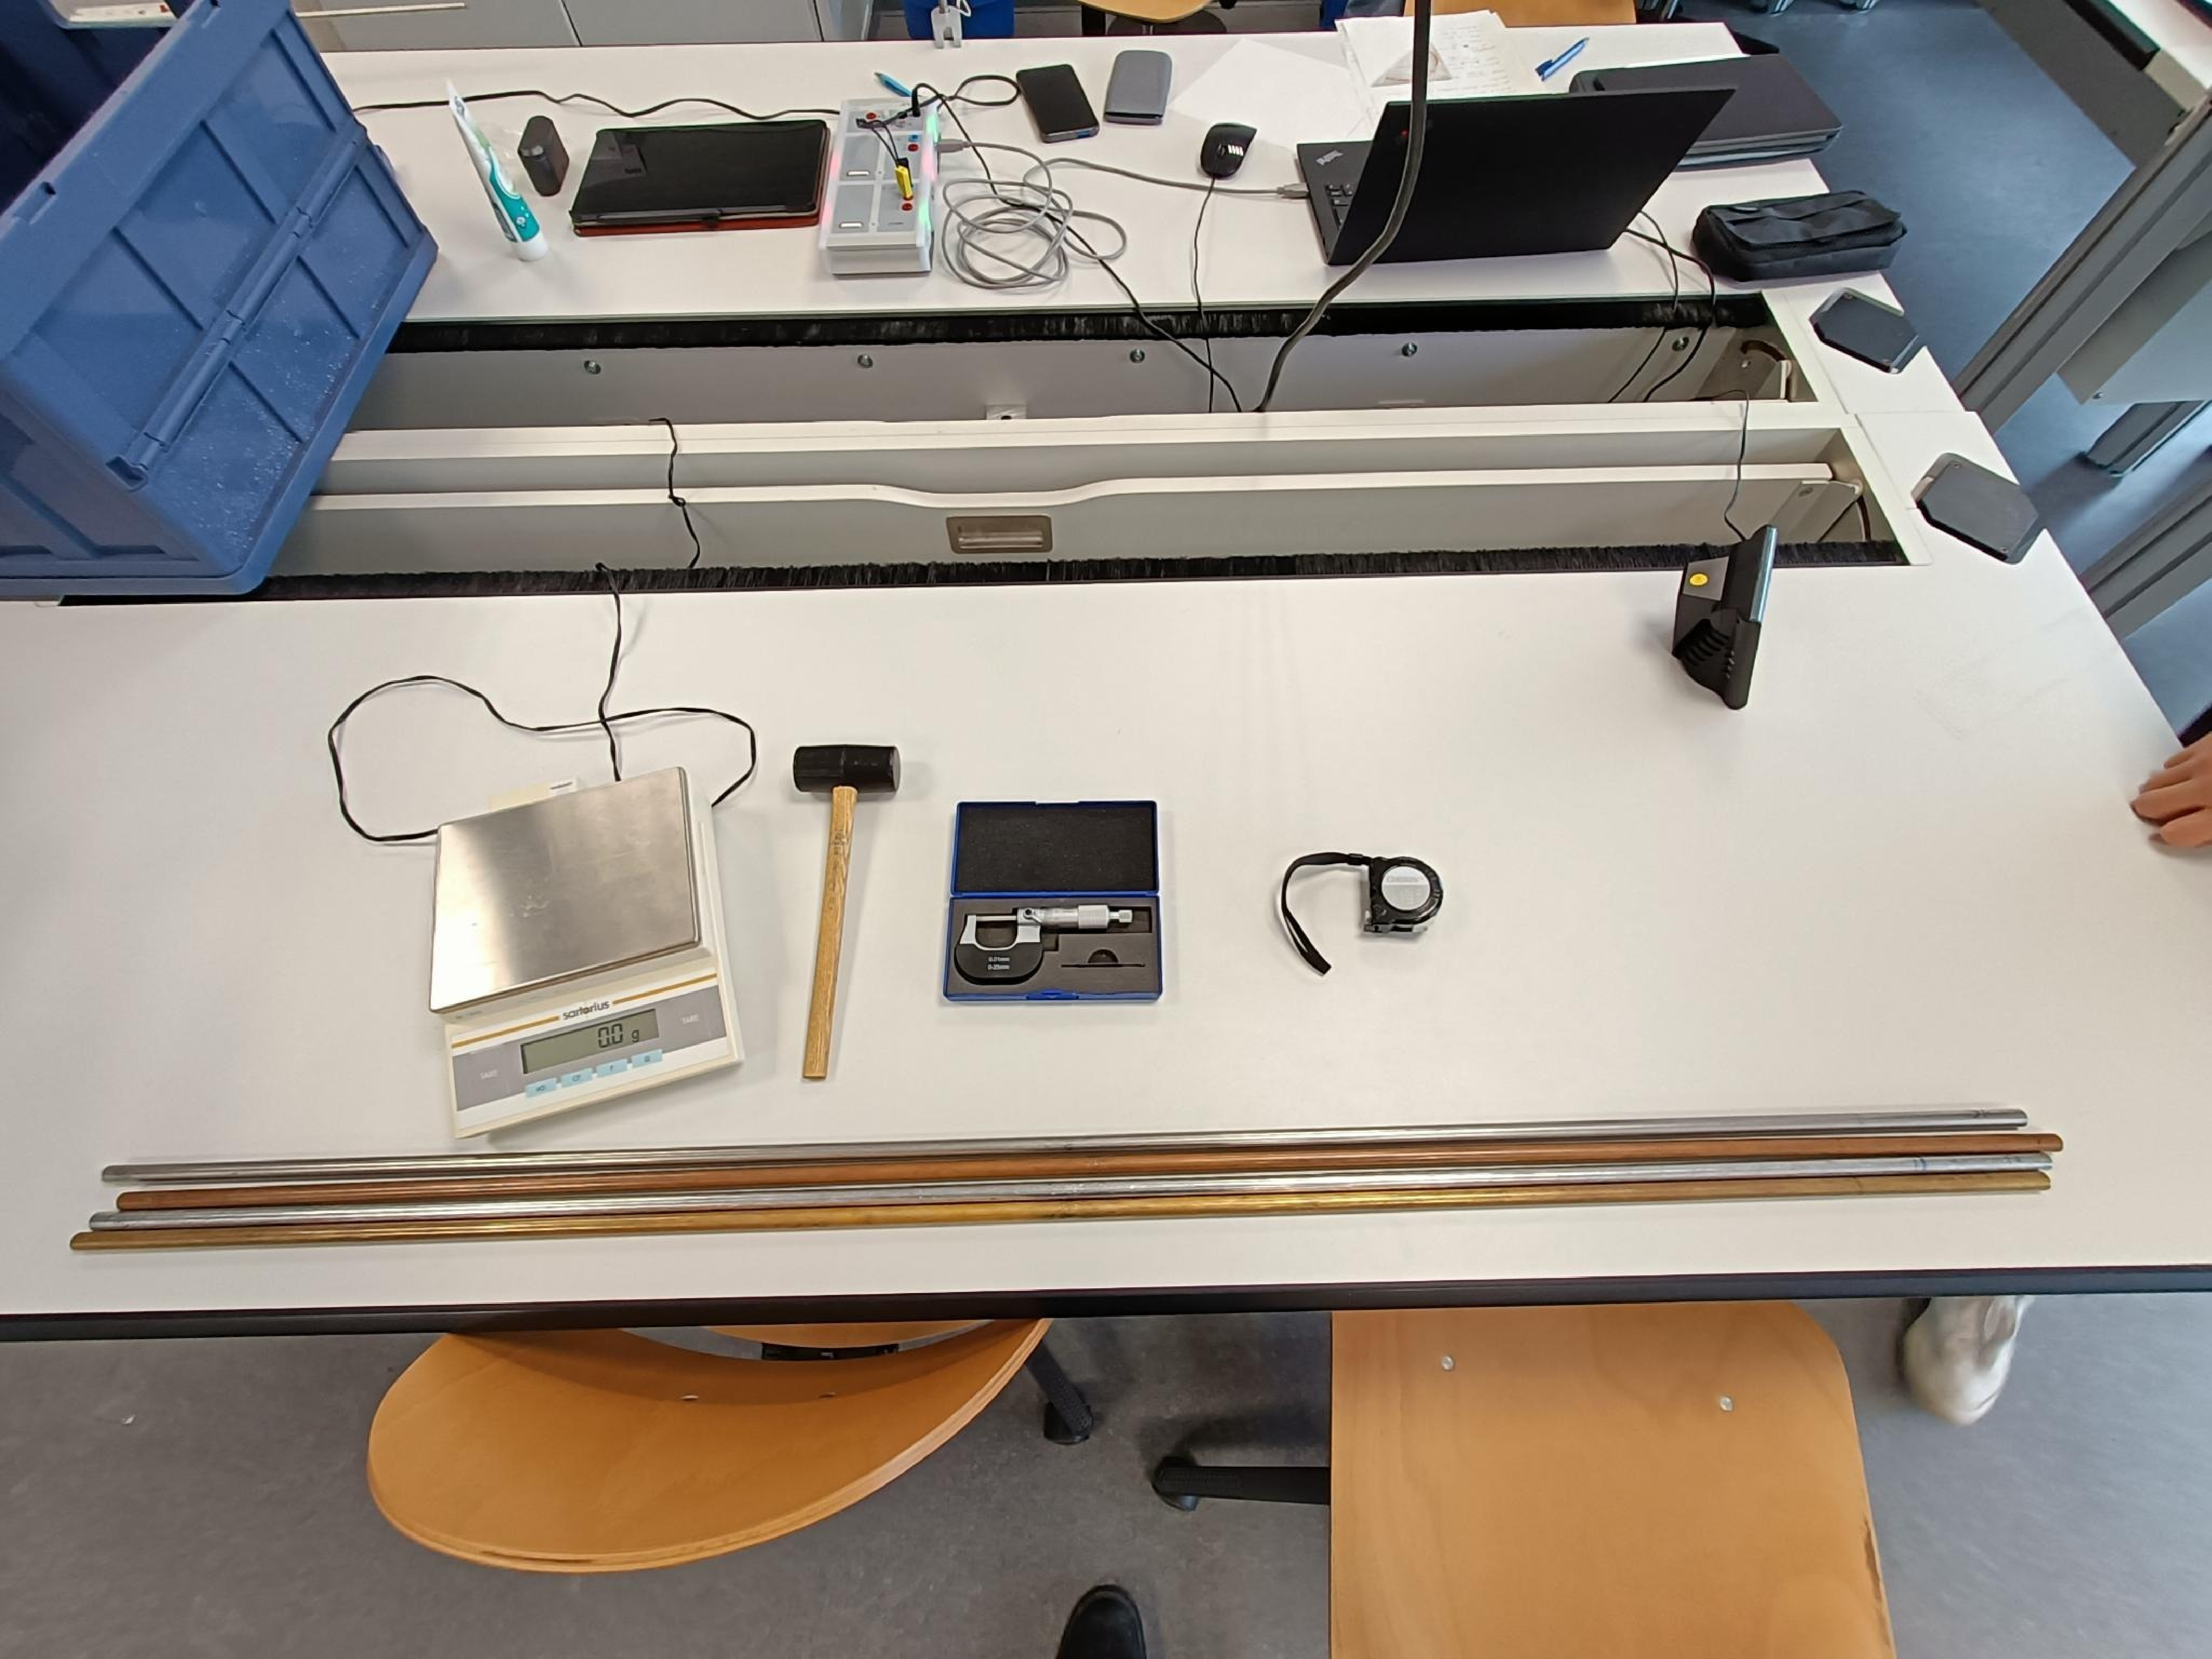
\includegraphics[width=0.3\textwidth]{Bilder/434170_428396_1A3_Materialien.pdf}\label{fig:f2}}
  \caption{My flowers.}
\end{figure}



Mit unseren eingestellten Messparametern haben wir dann eine erste vollständige Testmessung durchgeführt um zu überprüfen, ob alle Einstellungen gut passen. Aus dieser Messung haben wir erneut mit der FFT die Frequenz der Grundschwingung bestimmt. Mit dieser konnten wir eine erste Überschlagsrechnung für das E-Modul von Kupfer anstellen.
Diese ist im Messprotokoll zu finden. Da der Wert in der erwarteten Größenordnung lag, haben wir die Messreihe mit diesem Aufbau gestartet. 


Insgesamt haben wiir die Messung gleich wie bei der Testmessung 10 mal durchgeführt, und die Ergebnisse mithlife der FFT des CASSY Lab 2 grob auf konsistenz überprüft. Diese Messungen haben wir als unsere Messreihe abgespeichert.\\

Die Frequenz ist auch abhängig von der Einspannung der Stange, also von der Kraft und der position und der orientierung der Einspannung. Weswegen der Fehler aufgrund dieser Effekte auch beachtet werden muss. Dazu haben wir mit der Kupferstange Messungen durchgeführt bei denen wir die Einspannung um 1cm-2cm um den mittelpunkt variiert haben, sowie die Kraft mit der sie eingespannt ist, als auch die Rotation um die Längsachse.
Diese haben wir als Messreihe für spätere bestimmung des Fehlers gespeichert.\\

Das selbe Vorgehen wie bei der Kupferstange haben wir auch bei den anderen Stangen durchgeführt. Wobei wir jedes mal zunächst eine Testmessung gemacht habe, um die Empfinlichkeit des Mikrofons für das Material spezifisch ein zu stellen, und zu sehen ob die gemessene Frequenz, und damit auch das E-Modul den Erwartungen entspircht. 

Sämtliche gemessenen Daten haben wir gespeichert, sodass wir diese zur Auswertung verwenden können. einige Messungen mussten wir wiederholen, da wir die Stange nicht richtig angeschlagen hatten, oder sie sich beim Anschlag vom Mikrofon weggedreht hat. Ach durch Störgeräusche anderer Stangen, oder lautes Reden wurden einige Messungen gestört weswegen wir sie erneut durchführten.\\

Nach beendigung aller Messungen haben wir alles wieder abgebaut und an die dafür vorgesehenen Orte zurrückgelegt. 


\end{aufgabe}

\begin{aufgabe}{Rohdaten}

Der untenstehenden Tabelle können die Masse und die Länge der vermessenen Metallstangen entnehmen.  
    \begin{table}[H]
        \centering
        \begin{tabularx}{0.8\textwidth}{X c c} % adjust width as needed
            \toprule
            \textbf{Metall Stange} & \textbf{Masse} & \textbf{Länge} \\
            \midrule
            Aluminium & 460.9g & 150cm \\
            Messing & 1427.5g & 150cm \\
            Kupfer & 1505.4g & 150cm \\
            Stahl 15 & 1327.4g & 150cm \\
            \bottomrule
        \end{tabularx}
        \label{tab:mytable}
    \end{table}

In dieser Tabelle finden sie die Messung des Durchmessers. Diese haben wir pro Stange 10 mal durchgeführt. Gemessen wurde mit der Milimeterschraube an verschiedenen Positionen.
    \begin{table}[H]
        \centering
        \begin{tabularx}{0.8\textwidth}{X c c c c} % adjust width as needed
            \toprule
            \textbf{Messung} & \textbf{Aluminium} & \textbf{Messing} & \textbf{Kuper} & \textbf{Stahl 15} \\
            \midrule
            1. & 12.05mm & 11.98mm & 11.98mm & 12.00mm \\
            2. & 12.05mm & 12.01mm & 11.98mm & 12.00mm \\
            3. & 12.06mm & 11.98mm & 11.98mm & 11.99mm \\
            4. & 12.05mm & 11.99mm & 11.98mm & 12.00mm \\
            5. & 12.06mm & 11.98mm & 11.98mm & 12.00mm \\
            6. & 12.06mm & 11.98mm & 11.98mm & 12.00mm \\
            7. & 12.06mm & 11.99mm & 11.98mm & 12.00mm \\
            8. & 12.05mm & 11.99mm & 11.98mm & 12.00mm \\
            9. & 12.06mm & 11.98mm & 11.98mm & 12.00mm \\
            10.& 12.07mm & 11.98mm & 11.98mm & 12.01mm \\
            \bottomrule
        \end{tabularx}
        \label{tab:mytable}
    \end{table}
    

% schlechte Messungen:
    % Alu Messung 09 (Peak nicht gefunden, viel rauchen)
    % Kupfer einspann Fehler 3 (Peak nicht gefunden, viel rauchen)
    % Kupfer Messung 06 (Uebersteuern)
    % Kufper Einspann Fehler 06 (Peak nicht gefunden, viel rauchen)
    % Alu Messung 04 (Peak nicht gefunden, viel rauchen)
    % Alu Messung 02 (Peak nicht gefunden, viel rauchen)
    % Alu Messung 06 (Peak nicht gefunden, viel rauchen)
    % Stahl Messung 03 (Peak nicht gefunden, viel rauchen)
    % Kupfer Einsann Fehler 04 (Peak nicht gefunden, viel rauchen)
    % Alu Messung 07 (Peak nicht gefunden, viel rauchen)
    % kupfer Messung 10 (Peak nicht gefunden, viel rauchen)
    % Kupfer einsann fehler 05 (Peak nicht gefunden, viel rauchen)
    % Alu Messung 03 (Peak nicht gefunden, viel rauchen)
    % Alu Messung 05 (Peak nicht gefunden, viel rauchen)


% Gute Messung
    % Stahl Test 01
    % Stahl Messung 08
    % Kupfer Messung 01 (Gute abfall, man sieht störgeräusche) (Peak nicht gefunden)
    % Kupfer Einspann Fehler (Man sieht die abnahme gut)
    % Kupfer Test (Man sieht die abnahme gut)


% zu löschende Messungen:
    % Kupfer Einspann Fehler 05

% Graph von schlechter Messung, 
\end{aufgabe}

\begin{aufgabe}{Auswertung}

% TODO: Argumentiere, warum wir die peak methode mit range 1000 - 2000 nehmen, und nicht die peak_schwerpunkts methode.

  Bestimmen Sie aus den aufgezeichneten Schwingungsvorgängen die
  Schwingungsfreqünzen und tabellieren Sie die erhaltenen
  Werte. Ermitteln Sie die Streuung der einzelnen $f_i$ und bestimmen
  Sie daraus den statistischen Fehler auf den Mittelwert. Erläutern
  und illustrieren Sie Ihr Vorgehen zur Bestimmung der systematischen
  Unsicherheiten auf die Frequenz. Diskutieren Sie die Unsicherheiten
  auf $L$, $D$ und $M$. Berechnen Sie den E-Modul und die Dichte der
  vorliegenden Stangen und die zugehörigen statistischen und
  systematischen Messunsicherheiten. Diskutieren Sie, welche
  Fehlerbeiträge den Gesamtfehler dominieren. Vergleichen Sie Ihre
  Ergebnisse mit einschlägigen Literaturwerten.
\end{aufgabe}
 
\end{document}
